\documentclass[11pt,a4paper,oneside]{article}
\linespread{1.5}
\usepackage{amsmath,amsthm,amssymb,amsfonts,adjustbox,bm}
\usepackage{geometry}
\usepackage{threeparttable}
%\usepackage[dvipsnames]{xcolor}
\usepackage{mathtools}
\usepackage{refstyle}
\usepackage{pdflscape}
\usepackage{longtable}
\usepackage{eurosym}
\usepackage{enumerate}
\usepackage{booktabs}
\usepackage{siunitx}
\usepackage{rotating}
\usepackage{graphicx}
\usepackage{bbm}
\usepackage{subcaption}
\usepackage{caption}
\captionsetup{width=.8\textwidth}
\usepackage[section]{placeins}
\usepackage{xcolor}
\usepackage{geometry}
\usepackage{changepage}
\usepackage{float}
\usepackage[natbibapa]{apacite}
\usepackage{threeparttable}

\makeatletter
\NAT@longnamesfalse
\makeatother


\newcommand{\footremember}[2]{%
   \footnote{#2}
    \newcounter{#1}
    \setcounter{#1}{\value{footnote}}%
}
\newcommand{\footrecall}[1]{%
    \footnotemark[\value{#1}]%
} 
\usepackage{lineno}
\makeatletter
\def\makeLineNumberLeft{%
  \linenumberfont\llap{\hb@xt@\linenumberwidth{\LineNumber\hss}\hskip\linenumbersep}% left line number
  \hskip\columnwidth% skip over column of text
  \rlap{\hskip\linenumbersep\hb@xt@\linenumberwidth{\hss\LineNumber}}\hss}% right line number
\leftlinenumbers% Re-issue [left] option
\makeatother

\usepackage{blindtext}
\usepackage[colorlinks=true, citecolor=blue, linkcolor=blue, urlcolor=blue,breaklinks]{hyperref}

\linenumbers 


\title{Autoplay on Trial: An Online Experiment on the Suspect Behind Excessive Screen Time
% Commitment and autoplay videos: An online experiment
}
\author{Reha Tuncer\footnote{I am grateful to Ernesto Reuben and Kerstin Bongard-Blanchy for their guidance in the design and conception of this experiment, to Sophie Doublet for her help in interface design, to Suvadeep Mukherjee for his guidance in building web experiments. I am also thankful for the invaluable comments from the Behavioral Economics Summer School at the University of Copenhagen, the doctoral workshop at UC Louvain, the Experimetrics Workshop Soleto at Sapienza University Rome, Samuel Greiff, Manuel Munoz Herrera, Hande Erkut and countless colleagues.}}

\begin{document}

\maketitle


\section*{Abstract}

Interface design can `nudge' consumers to take certain actions and is suspected of promoting addictive online behavior. A prevalent interface element across popular social media and streaming platforms is the default autoplay feature. We present an incentivized two-day online experiment to investigate whether the autoplay feature alone can cause an increase in undesired video consumption. We recruited 184 participants who allocated time between transcription tasks and watching funny animal videos, randomly assigning them to either autoplay or click-to-play video conditions while holding content constant. We find that the autoplay feature, in isolation, does not override participants' previously indicated preferences for media consumption. Participants exhibited positive willingness-to-pay for autoplay (2.24 pence on average), viewing it as a convenience feature rather than a self-control problem. However, experimenter demand effects have hampered with the intended autoplay manipulation. These findings highlight the importance of ecological validity in studying interface design effects on user behavior.

\section{Introduction}

Autoplay is a user interface feature which automatically transitions users to new video content without any action. It has become a familiar design element in major social media and streaming platforms over the last decade,\footnote{As of 2025 these platforms include Facebook, Instagram, Netflix, YouTube, TikTok, and Twitter (currently X). Twitter \href{https://blog.x.com/official/en_us/a/2015/introducing-a-more-seamless-video-experience-with-autoplay.html}{first introduced} autoplay in 2015, and described it as a means to reduce ``extra effort'' in the number of clicks/taps required to consume content.} and has been described as a default nudge that reduces the autonomy of users \citep{lukoff2021design,schaffner2025pahi}. Autoplay's widespread adoption and concerns about its restricting the freedom of choice has also attracted regulatory scrutiny, with the U.S. SMART Act proposing to ban platforms from serving autoplay content ``without an express, separate prompt by the user'' due to suspicions of its contribution to addictive online behavior.\footnote{\href{https://www.congress.gov/bill/116th-congress/senate-bill/2314/text}{SMART Act of 2019}, S. 2314, 116th Congress.}

While autoplay is pervasive and tends to increase viewing times \citep{chen2025,hiniker2018coco,schaffner2025pahi}, its impact on user welfare and the mechanisms driving this effect are not well understood. Does the increase in consumption go against users' wishes, or does it merely remove frictions to help them achieve their desired consumption levels? Can we attribute the increase in consumption to autoplay in isolation, or does it also depend on the supply of content? One reason for these gaps is the challenge of holding constant the video content displayed to users while eliciting their preferences related to content consumption before the actual consumption occurs.

We overcome this challenge in an incentivized two-day online experiment designed to isolate the causal effect of autoplay on content consumption. We recruited 184 participants who twice allocated 1200 seconds (20 minutes) between two tasks. The tasks involved seconds of transcription of random character sequences texts at 0.15 pence/second, and seconds of watching funny animal videos at 0.1 pence/second. On the first day, participants got familiar with tasks and made hypothetical allocations using the strategy method. On the following day, participants realized their time allocation decision without constraints. This two-day structure with hypothetical and realized choices formed the foundation for testing our preregistered hypotheses regarding autoplay.

To isolate the causal effect of autoplay on these allocation decisions, we randomly assigned participants to either the \textit{Autoplay} or \textit{Control} condition. In the \textit{Autoplay} condition watching task videos played continuously. In the \textit{Control} condition participants explicitly clicked to play each video. We held constant the content by presenting 80 manually curated ``funny animal'' videos from YouTube and TikTok in identical sequence. This eliminated algorithmic content curation and personalization as potential confounds. We dedicated the first block of the experiment to measure the differences between planned and realized allocations across conditions.

In a second block of the experiment, we modified the design to elicit demand for a commitment device. We recruited 52 additional participants who made nine binary choices: they could either keep their preferred autoplay setting (on or off) or switch to the opposite setting in exchange for bonus payments ranging from £0.05 to £0.50. We implemented one of these decisions at random, determining both the autoplay setting for the next day and the associated bonus payment. This allowed us to measure participants' Willingness To Pay (WTP) for autoplay in advance, providing insight into whether participants viewed the feature as beneficial (positive WTP) or as a self-control problem requiring a commitment device (negative WTP).

We report three key findings. The first set of results focuses on our preregistered hypotheses regarding  autoplay. We find no evidence that autoplay in isolation increased content consumption. Participants in the \textit{Autoplay} condition watched statistically indistinguishable numbers of videos compared to the \textit{Control} condition. \textit{Autoplay} condition also had no significant effect on the proportion of time spent on either task. These results also hold for other engagement metrics (i.e., average session length, number of sessions).

Second, participants viewed autoplay as beneficial rather than problematic. Contrary to our hypothesis that participants would demand commitment devices against autoplay, we find a positive WTP for the feature. Using data from the second block, we are able to estimate an average WTP of 2.24 pence (about 45 seconds of transcribing) for the 20-minute session. Autoplay is considered as a convenience feature rather than as a threat to self-control, aligning with earlier research \citep{bongard2021definitely,schaffner2025pahi}.

Third, participants consumed less content than initially planned. Comparing hypothetical time allocations to realized ones, we find that participants consumed significantly less content than their day 1 plans implied in both conditions. The decrease amounts to 15.8 percentage points (35\%) less time spent on the watching task. This result is driven by 33\% of all participants who had planned to spend up to three quarters of their time watching videos but instead decreased their content consumption on the next day. On the other end, 88\% of those who had initially planned to spend less than a quarter of their time watching videos successfully followed their plans and did not succumb to temptation.

Evidence from a regression discontinuity analysis shows that participants monitored their day 1 plans despite ultimately exceeding them. When participants reached their planned transcribing duration, they immediately reduced transcribing probability by 25.5 percentage points in the next 60-second window. However, this effect dissipated quickly and became statistically insignificant within 90 seconds as participants resumed transcribing. 

Taken together, these findings cast doubt on whether the watching task was actually perceived as tempting. A mixed-methods analysis of open-ended responses reveals that participants perceived the experimental environment as a work setting rather than a choice between independent tasks. While 29\% spontaneously described transcribing using negative terms, another 23\% characterized video-watching as ``taking breaks'' from work. This suggests that experimenter demand effects may have interfered with the intended effects of the autoplay manipulation, with implications for both the interpretation of our null results and the broader generalizability of our study.

A primary internal validity concern is that experimenter demand effects favored allocating more time to the transcribing task than planned. These can emerge through contextual cues even without explicit behavioral instructions, as participants interpret the unfamiliar experimental environment by drawing inferences from the information provided. They may alter behavior simply by having attention drawn to variables of interest \citep{zizzo2010ee}. In our experiment, these could be (i) the small earnings difference favoring the transcribing task,\footnote{This difference is 60 pence over 20 minutes, equivalent to a 1.8 pound hourly wage difference (15\% above our 12 pound minimum wage baseline).} (ii) multiple mentions of the quality criteria for the transcribing task to receive earnings, (iii) placement of the transcribing task as the first activity upon starting a session. Alternative designs could have addressed these concerns by rewarding balanced time allocations more, or by eliminating earning differences altogether.

Another major challenge in isolating the effects of autoplay is the role of content appeal. Higher content appeal would make the watching task more tempting, and create a stronger tradeoff between the two tasks. To address this while keeping the content identical across conditions, we conducted pretests from the same participant pool where the funny animal videos came out as the most popular theme. Participants also rated the curated videos positively (median 7/10) in a post experiment survey. Regardless, the watching task content may not have been sufficiently appealing. Allowing participants to select among a list of themes with manually curated videos could have addressed this issue \citep{ek2023too}.

A final concern in online experiments is ensuring genuine participation equivalent to laboratory conditions. We implemented several measures to address this challenge. We used JavaScript-based attention monitoring to detect each second participants navigated away from the experimental interface following \citep{purohit2023starving}. We also required minimum internet speeds and restricted participation to desktop users with Chromium-based browsers to standardize the user experience. Participants also answered post-experiment survey questions about their engagement while watching videos and about connection interruptions. These controls ensured that our final dataset is composed of participants who were active, and  approximate the controlled conditions of laboratory experiments \citep{arechar2018conducting}.

We contribute to several strands of literature. First, the literature on studying the effects of social media and streaming services on user well-being \citep{nyhan2023like,allcott2022digital,allcott2020welfare, collis2022po, groshek2018p9icsms, walton-pattison2018jhp, braghieri2022aer,bursztyn2023,beknazar2025toxic,purohit2023starving,nyhan2023like,bao2025just}. We contribute to this work by shedding light on one potential driver of the harmful effects of social media and streaming services, the autoplay, in a controlled setting.

A subset of this literature focuses on the effects of specific interface design elements on user behavior, particularly related to user agency and overconsumption of content \citep{lukoff2021design,bongard2021definitely,schaffner2025pahi,schaffner2023pahia, mathur2021p2cchfcs, lyngs2019p2cchfcs, lyngs2020p2cchfcs, silverman2024, lupianez-villanueva2022, chen2025,hoong2021eer}. To our knowledge, our paper provides the first attempt at isolating the causal effects of autoplay on content consumption.

Methodologically, this paper contributes to the literature on laboratory experiments that observe behavior in real time while participants trade cognitive effort with leisure \citep{kool2014labor,bhatia2021,ek2023too,bonein2015ee,houser2018gaeb}. We also add to a burgeoning literature manipulating design elements within the user interface to reduce overconsumption of content \citep{hiniker2018coco,lyngs2020p2cchfcs,purohit2023starving,schaffner2025pahi}.

The remainder of this paper is organized as follows. Section \ref{Design} describes the experimental design. Section \ref{SandP} details the experimental sample and procedures. Section \ref{Results} presents our results and Section \ref{Conclusion} concludes.

\section{Design}\label{Design}

\subsection{Timeline and Session Structure}
We conducted a two-day online experiment to examine how autoplay feature affects time allocation between transcription of random character sequences and watching funny animal videos. The multi-day structure allowed us to measure the gap between stated preferences and actual behavior under two different video interface conditions. Participants completed two separate data collection sessions with a cooling-off period of 24 hours (up to 48 hours) between sessions.

Day 1 sessions included a practice session to familiarize participants with the experimental interface, followed by preference elicitation measures. Day 2 featured the main 20-minute session where participants made actual time allocation decisions. We conducted two waves of data collection during May 2023, as described in Table \ref{summary_table}.

\begin{table}[H]
\centering
\begin{threeparttable}
\caption{Summary of experimental design and timeline}
\begin{tabular*}{\textwidth}{@{\extracolsep{\fill}} l c c c c c @{}}
\toprule
& \begin{tabular}[c]{@{}c@{}}Practice\\ Session\end{tabular} & \begin{tabular}[c]{@{}c@{}}Time\\ Choice\end{tabular} & \begin{tabular}[c]{@{}c@{}}Main\\ Session\end{tabular} & \begin{tabular}[c]{@{}c@{}}Multiple\\ Price List\end{tabular} & \begin{tabular}[c]{@{}c@{}}Decision\\ Horizon\end{tabular} \\
\midrule
Day 1 (May 10) & \checkmark & \checkmark &  &  & 24-hour \\
Day 2 (May 11) &  &  & \checkmark &  & immediate \\ \midrule
Day 1 (May 18) & \checkmark & \checkmark &  & \checkmark & 24-hour \\
Day 2 (May 19) &  &  & \checkmark &  & immediate \\
\bottomrule
\end{tabular*}
\begin{tablenotes}[flushleft]
\footnotesize
\item[] \textit{Note:} This table shows the experimental components administered across two data collection waves, with columns ordered chronologically within each day. The first block (May 10-11 2023) established baseline effects, while the second block (May 18-19 2023) incorporated the Multiple Price List to measure demand for a commitment device. Decision horizon refers to the time between hypothetical preference elicitation and the main experimental session.
\end{tablenotes}
\label{summary_table}
\end{threeparttable}
\end{table}

\subsection{Technical Implementation and Interface Design}
We designed the experimental platform to provide precise control over the testing environment while maintaining ecological validity. We presented both tasks within a single web page using distinct tabs, allowing participants to switch between activities seamlessly while preserving progress. Sessions began with the transcription task as the default, requiring an active choice to switch to the watching task.

The interface incorporated several key features to track behavior. A progress bar and timer provided real-time feedback on session duration. We logged all critical interactions including tab switches, keystrokes during transcription, video controls, and cursor movements outside the experimental window. This granular tracking enabled us to construct detailed measures of attention and engagement across tasks.

\subsection{Internal Validity Controls}\label{int-val}
Online experiments present unique challenges for maintaining experimental control, including participant multitasking, technical disruptions, and environmental variation. We implemented comprehensive measures to address these concerns and ensure data quality.

\textbf{Participant and Technology Screening:} We selectively admitted participants using multiple screening criteria to ensure stable experimental conditions. Internet speed requirements filtered out participants with unstable connections (minimum 30 Mbps on day 1, 25 Mbps on day 2). We restricted participation to users with Windows, Linux, or Mac operating systems using Chromium-based browsers exclusively. We excluded Safari and Mozilla Firefox due to restrictive autoplay configurations. Mobile devices and tablets were prohibited to standardize the user experience.

\textbf{Platform Controls:} The experimental website enforced linear navigation, preventing participants from moving backward through the experiment. We disabled right-click functions and keyboard shortcuts. Any attempt to navigate backward reset progress to the landing page. We clearly communicated these restrictions to participants at the experiment's outset.

\textbf{Attention and Engagement Monitoring:} We implemented real-time tracking of participant attention using a JavaScript library to detect interface visibility disruptions.\footnote{See more information about the \href{https://developer.mozilla.org/en-US/docs/Web/API/Intersection_Observer_API}{Intersection Observer API}.} This system captured actions such as minimizing the browser, switching between web pages, or launching other applications. The tracking provided second-by-second accountability of participant engagement.

\textbf{Post-Experiment Validation:} After completing the experiment, participants reported any connectivity disruptions and confirmed their genuine engagement with the watching task. We combined these self-reports with our objective tracking measures to identify and filter data potentially compromised by distractions or divided attention.

\subsection{Tasks}
\subsubsection{Transcription Task}\label{transcription-task}
The transcription task requires transcribing successive CAPTCHAs. CAPTCHAs are computer-generated images that contain random letters, numbers and randomly placed white spaces.\footnote{We added white spaces to improve readability after pretests. The number of white spaces was limited to a maximum of 5 instances per CAPTCHA to control the transcribing time per image.} Each CAPTCHA has a total length of 35 characters, including the white spaces. Participants spent on average 41 seconds per CAPTCHA.

We designed the images to be blurred and distorted by lines and dots added on top to increase comprehension difficulty.\footnote{The \href{https://osf.io/2vqwf/?view_only=1ef589ec2e544db4ad9b6ab9c45ff849}{randomization procedure} to generate CAPTCHAs.} The interface always presents these CAPTCHA images with a text box and a submit button. When the submit button is clicked, the next CAPTCHA image appears and the text input for the previous one is stored. The task is identical across conditions, as illustrated in Figure \ref{transcription-screen}.

We established easy-to-meet quality requirements to ensure participants remained active. These requirements include an overall transcription accuracy of at least 70 percent in submitted CAPTCHAs\footnote{We use Python's \href{https://docs.python.org/3/library/difflib.html}{\texttt{difflib}} string-matching algorithm to measure accuracy. It consists of finding the longest common substring and then finding recursively the number of matching characters in the non-matching regions on both sides of the longest common substring. Overall accuracy of 70 percent implies an average of 10.5 ($0.3*35$) mistakes across all submitted CAPTCHAs.} and a minimum of one CAPTCHA submission per minute spent on the task. Participants had to meet these quality requirements to receive compensation for the transcription task.


\begin{figure}[H]
   \caption{Transcription task tab}
    \centering
       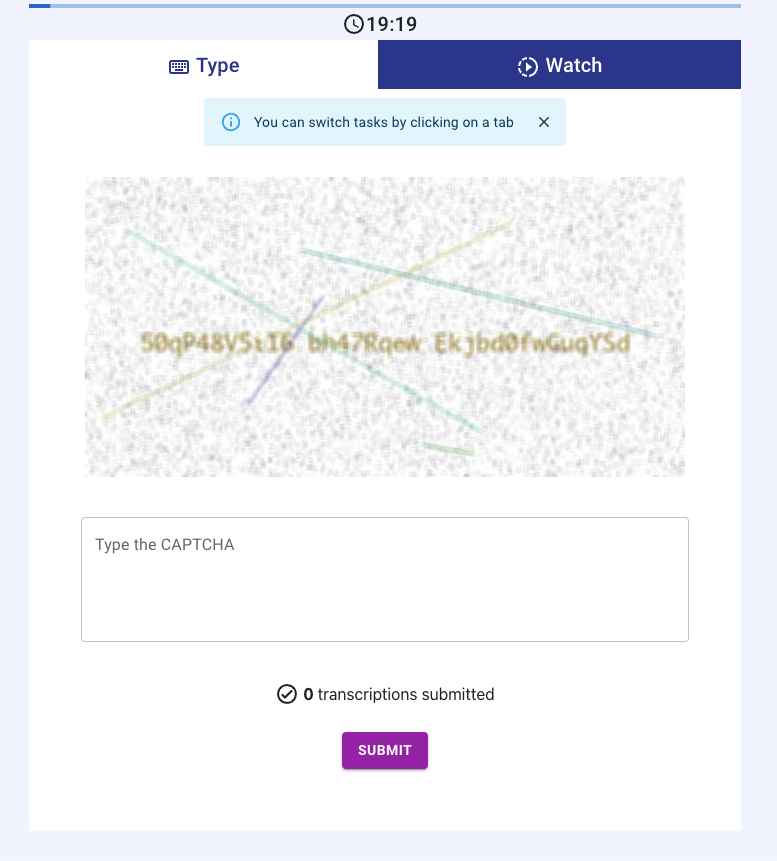
\includegraphics[width=0.6\linewidth]{typing.png}
   \label{transcription-screen}
   \begin{tablenotes}
   \footnotesize
\item[] \textit{Note:} This figure describes the transcription interface tab. As participants always begin in the transcription tab by default, there is a banner that reminds participants to click the tab buttons to switch tasks. This banner disappeared as soon as participants switched tasks once.
\end{tablenotes}
\end{figure}

\subsubsection{Watching Task}\label{watching-task}
In this task, participants watch successive short videos in a customized media player. Since we are interested in isolating the media player's default settings, the video content and the order in which videos appear to participants are identical across conditions. We completely disabled the media player controls: Participants cannot skip videos (user scrolling is disabled) or use the media player's slider to advance or go back in a particular video.

The conditions differ in their autoplay functionality. In the \textit{Autoplay} condition, videos play automatically when the watching tab is visible and pause with a click anywhere on the video. While the watching task is visible, the media player keeps scrolling to the next videos and continues playing them unless interrupted. In the \textit{Control} condition, participants need to have the watching tab visible and click on each consecutive video to play them. At the end of each video, the scrolling animation brings the next video, but the new video only starts playing when the participant clicks on it. Figure \ref{watching-screen} illustrates the video tab in the \textit{Control} condition.

We manually selected 80 videos to isolate the difference in the media player design and help avoid algorithmic biases resulting from the recommender system's personalized suggestions. We curated videos from YouTube and TikTok, using the tags ``funny animal'' and ``cute animal''.  We chose animal videos because of their popularity during pilot studies.\footnote{During the pilots, the experiment was followed by a separate questionnaire asking participants to rate the videos they had seen and suggest what types of videos they would have liked to see more of.} We reviewed the selected videos to ensure that they did not contain any harmful or violent actions toward the animals involved. We kept the first 60 videos shorter in the beginning to maximize the frequency of experiencing the autoplay feature during the watching session, with videos getting longer for the last 20 videos (see Table \ref{tab:video_duration}).

\begin{table}[H]
  \centering
  \caption{Video durations in the watching task}
  \begin{threeparttable}
  \begin{tabular*}{\textwidth}{@{\extracolsep{\fill}}lccc}
  \toprule
  & \multicolumn{1}{c}{\textbf{First 60 videos}} & \multicolumn{1}{c}{\textbf{Last 20 videos}} \\
  \midrule
  \textbf{\textit{Duration (seconds)}} & & \\
  Mean (SD) & 12.25 (7.04) & 25.50 (14.04) \\
  Median [Min, Max] & 10 [5, 38] & 19.5 [8, 60] \\
  \bottomrule
  \end{tabular*}
  \begin{tablenotes}[flushleft]
  \footnotesize
  \item[] \textit{Note:} This table presents the duration characteristics of the 80 animal videos used in the experiment. The first 60 videos were kept shorter to maximize participants' exposure to the autoplay feature during watching sessions, while the last 20 videos were longer. 
  \end{tablenotes}
  \end{threeparttable} \label{tab:video_duration}
\end{table}

\begin{figure}[H]
   \caption{Watching Task tab}
    \centering
       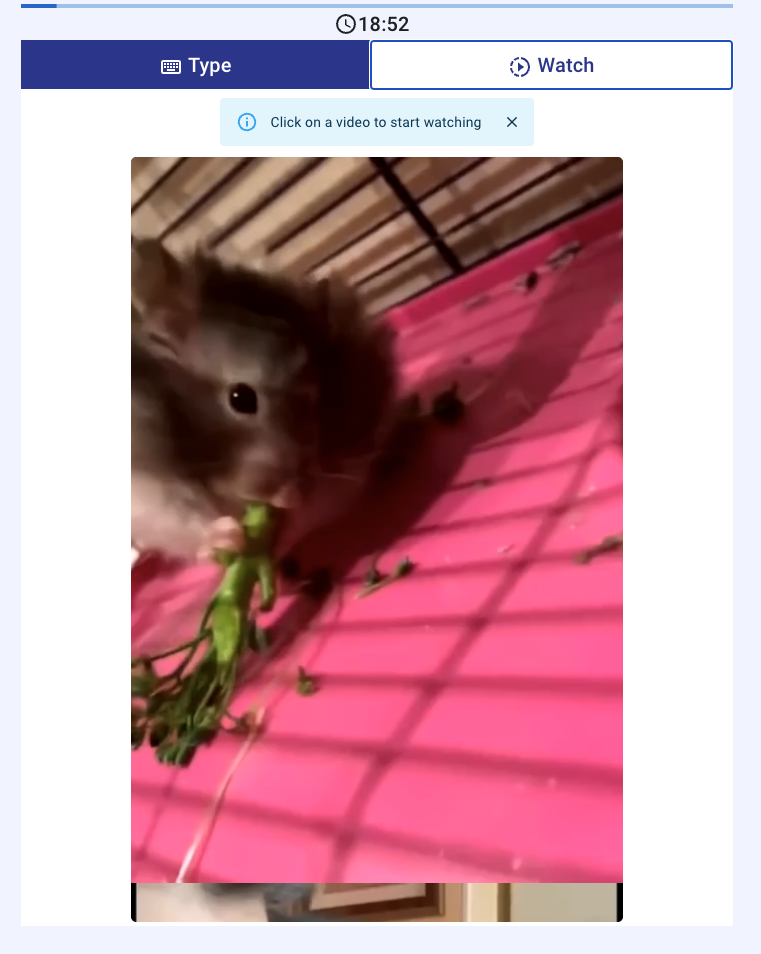
\includegraphics[width=0.6\linewidth]{watching.png}
   \label{watching-screen}
   \begin{tablenotes}
\footnotesize
\item[] \textit{Note:} This figure describes the ``Watch'' tab in the \textit{Control} condition. Before the first video is clicked upon to be played, there is a banner that reminds participants that the video won't play without clicking. This banner was not present in the \textit{Autoplay} condition and videos started playing as soon as participants clicked on the ``Watch'' button seen up on the right. Notice that the top part of the following video is already visible in the bottom part of the screen.
\end{tablenotes}
\end{figure}

\subsection{Practice Session}\label{practice}
The experiment consists of two sessions during which participants interact with the tasks described above. The first session is the practice session on day one. It comes right after the written descriptions of each task and serves to familiarize participants with the tasks and the interface. Participants are assigned to either \textit{Autoplay} or \textit{Control} condition before the practice session, so that they experience the same video interface on both the Practice and Main Sessions.

During the practice session, each task was available for only 60 seconds and participants were not allowed to switch between tasks. On the first tab, participants were required to retype CAPTCHAs. The 60-second period was enough to submit one CAPTCHA and see the second CAPTCHA image. After 60 seconds, a pop-up appeared on the screen blocking any other interaction and taking participants to the second page.

Participants were required to close this pop-up to advance to the second task. The rationale behind the pop-up was to ensure participants spent equal time on both tasks. Whether or not this pop-up was closed was verified to check participant activity and served as an additional attention check.\footnote{All participants closed this pop-up and switched to the watching task.} Once closed, the watching task began for 60 seconds, enabling participants to watch 4 to 5 short videos depending on whether they were assigned to the \textit{Autoplay} or the \textit{Control} condition. In the \textit{Autoplay} condition, videos played continuously, while in the \textit{Control} condition, videos required a click to start.

We did not remunerate participants for the time they spent here because the purpose of the practice session was to understand the difficulty and pacing of the tasks, as well as navigation within the interface.

\subsection{Multiple Price List}\label{mpl}
In the second block of the experiment, participants made 9 binary decisions (see Figure \ref{mpl-screen}). These decisions were made after the practice session on day one. Participants chose between their preferred media player setting (autoplay off or on) and a bonus payment. We determined bonuses by the per-second earning differences across tasks, multiplied by the expected differences in time spent between the conditions in the first block of the experiment. 

Specifically, we expected the average difference between the \textit{Autoplay} and \textit{Control} conditions, in terms of time spent across tasks, to be in the magnitude of 60 seconds (it was 79.5 seconds, from Table \ref{table3}). This resulted in an average earning difference of $60*(0.15-0.1)=3$ pence. To capture this in the MPL choices offered, we set the symmetric bonuses accordingly: £[0.05, 0.1, 0.25, 0.5].

Once these decisions were completed, we randomly implemented one of their 9 choices and informed participants whether autoplay would be on or off, and of their associated bonus earnings. With this knowledge, participants then made their hypothetical time allocation for day 2.

\begin{figure}[H]
    \caption{Multiple Price List page}
   \centering
       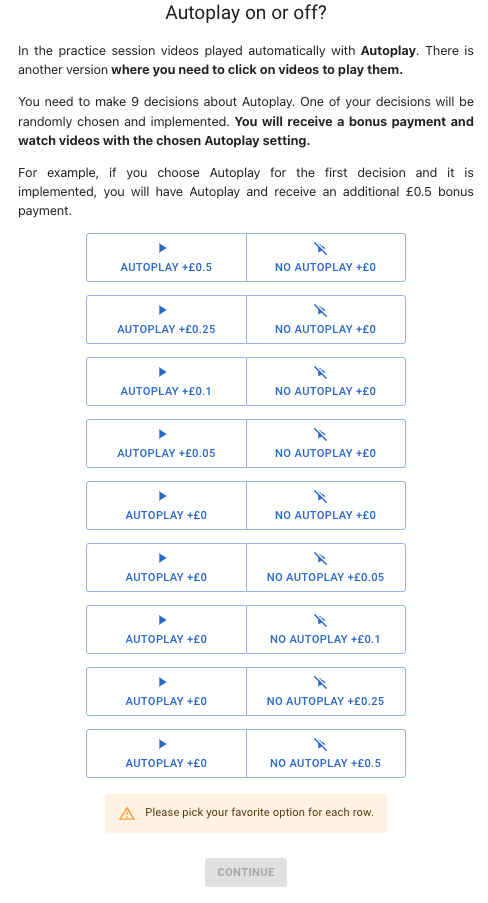
\includegraphics[width=0.6\linewidth]{mpl.png}
   \label{mpl-screen}
      \begin{tablenotes}
\footnotesize
\item[] \textit{Note:} This figure describes the MPL page where participants made 9 binary choices between their preferred autoplay setting and bonus payments. Each row presents a choice between ``Autoplay'' (left) and ``No Autoplay'' (right) with associated bonus amounts ranging from £0.05 to £0.5. The interface required participants to select one option in each row before proceeding. One of these 9 decisions was randomly selected for implementation in the Main Session, determining both the autoplay setting and any bonus payment for day two.
\end{tablenotes}
\end{figure}

\subsection{Time Choice}\label{time-choice}
Following the practice session, participants transitioned to the time choice section. This section required them to specify their preferred time allocation between the two tasks for the following day. Participants were informed the main session would be 20 minutes long and they were free to choose corner solutions, even if that meant focusing solely on one task.

We designed a slider tool with 20-second steps for participants to indicate their time allocation preferences. Initially, the slider appeared grayed out and required a click to activate. This design aimed to ensure participants considered their choices in an active manner. The click-to-activate design had two benefits: It guaranteed participants interacted with the slider and helped participants understand the task-related payoff structure.

To incentivize this decision, we randomly made 5\% of the day 1 choices binding in the main session. Binding choices led to payments based on the initial time choice, but only if participants met the quality standards described under Section \ref{transcription-task} during day 2. We excluded data from these participants from the final dataset accordingly. We informed participants whether their allocation was binding with their time choice reminder on day two, right before the start of the main session.

The time choice served as a benchmark for participants, and participants accordingly received a reminder of it on day two. The time choice section offers insights into participants' informed time preferences and allows verifying their commitment to these choices after a 24-hour period.

\begin{figure}[H]
    \caption{Time Choice page}
   \centering
       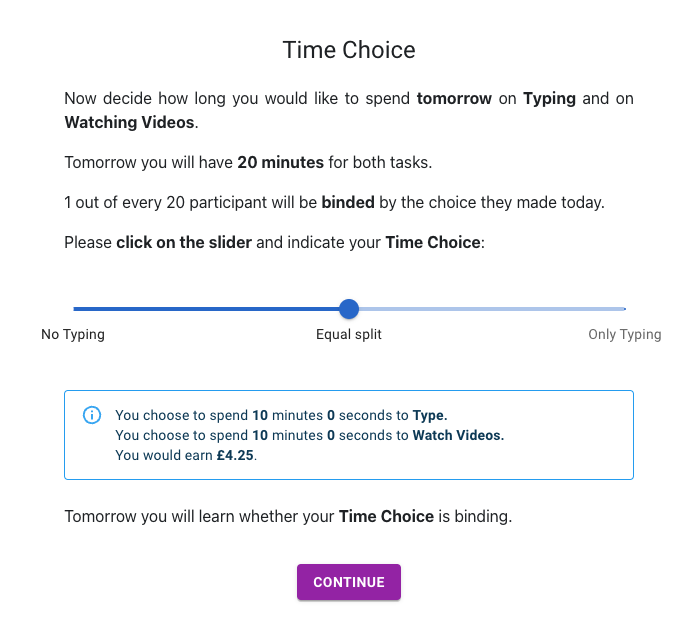
\includegraphics[width=0.6\linewidth]{time-choice.png}
   \label{time-choice-screen}
   \begin{tablenotes}
\footnotesize
\item[] \textit{Note:} This figure shows the time choice interface with a slider tool allowing participants to allocate time between the two experimental tasks for the following day's 20-minute main session. The slider initially appears grayed out and requires a click to activate. Real-time feedback shows the selected allocation (here, 10 minutes each) and expected earnings (£4.25). The interface informs participants that 1 out of 20 (5 percent) will be bound by their choice and that they will learn whether their choice is binding on day two.
\end{tablenotes}
\end{figure}

\subsection{Main Session} \label{main-session}

The main session took place on day two, approximately 24 hours after the time choice. We began by reminding participants of their previous day's time allocation and informing them whether their time choice was binding. 95\% of participants were free to allocate their time on day 2 as they preferred.

The main session lasted 20 minutes. Participants could freely switch between the transcription and watching tasks at any time using the tab interface. Unlike the practice session, there were no time restrictions on individual tasks. Participants had complete autonomy over their time allocation decisions. The interface maintained real-time tracking of time spent on each task, and participants could monitor their time allocation through the progress bar and a timer.

We implemented the experimental treatment during this session through the media player's autoplay functionality. Participants assigned to the \textit{Autoplay} condition experienced continuous video playback when the watching tab was visible, while those in the \textit{Control} condition required a click to start each video.


\subsection{Hypotheses}\label{hypotheses}
User interface design choices are ``not separable from other content choices, since their effect depends on where the platform has positioned its content on the underlying content manifold.'' \citep{kleinberg2022challenge}. If content has very low inherent appeal and stickiness, autoplay may have minimal effect on video consumption. An analogy is how introducing breaks would have little impact on engagement for low-stickiness content like documentaries, but dramatically reduce engagement for high-stickiness content like celebrity gossip.\footnote{See \citet{bao2025just} for recent work on addictive short drama series.} 

Assuming that our selection of videos have sufficient appeal and stickiness, \textit{Autoplay} condition should lead to consumption beyond users' stated preferences, creating a measurable gap between hypothetical time choice and actual behavior. In this case, we expect autoplay's behavioral effects to be known by participants, albeit underestimated as to how much they would be affected by these interfaces \citep{bongard2021definitely}. We thus expect positive demand for a commitment device driven by ``sophisticated'' participants in line with time preference literature \citep{ericson2018}. 

\textbf{Hypothesis 1:} \textit{Autoplay} condition decreases time allocated to the transcription task while increasing video consumption. We test this using a linear regression:
\begin{equation}\label{eq1}
Y_{i} = \alpha + \gamma \text{Autoplay}_{i} + \beta \text{TimeChoice}_{i} + \delta (\text{Autoplay}_{i} \times \text{TimeChoice}_{i}) + \epsilon_{i}
\end{equation}
where $Y_{i}$ represents our outcome variables of interest (proportion of time spent on transcription or number of videos watched), $\text{Autoplay}_{i}$ is a binary indicator for the condition, and $\text{TimeChoice}_{i}$ is the standardized proportion of time participants planned to spend on transcription on day 1. We estimate this model with and without the interaction term to examine whether the autoplay effect varies based on initial planning preferences. We expect $\gamma < 0$ for transcription and $\gamma > 0$ for videos watched.

\textbf{Hypothesis 2:} \textit{Autoplay} condition has an effect on deviations from stated time allocation preferences (actual minus planned time spent on transcription). We test this using a two-sample $t$-test comparing the means between the two conditions.

\textbf{Hypothesis 3:} If participants are aware of their self-control issues, they should exhibit negative Willingness To Pay (WTP) for autoplay, preferring the commitment devices that restrict automatic video transitions. We test this using a logistic regression:
    \begin{equation}\label{eq2}
        {Y}_{ij} = \alpha + \beta \text{Bonus}_{ij} + \epsilon_{ij}
    \end{equation}
where ${Y}_{ij}$ is the binary choice of taking autoplay given the bonus $j$ from the MPL for individual $i$. We calculate the WTP for autoplay as the population-averaged effect of bonus $-\alpha/\beta$, and expect a negative sign indicating preference for commitment against autoplay.

In sum, these hypotheses test whether interface design features can systematically distort optimal time allocation decisions in a setting where participants face clear monetary incentives favoring the transcription task.\footnote{\href{https://doi.org/10.17605/OSF.IO/MFKBC}{Access} the preregistered hypotheses. Our preregistration included hypotheses 1 and 3. We have added supporting hypothesis 2 regarding our expectations about the time choice section later.}


\section{Sample and Procedures}\label{SandP}
The experiment was run entirely online, using widely available open-source tools.\footnote{We used the \href{https://www.mongodb.com/languages/mern-stack-tutorial}{MERN stack} to develop and host the website in an entirely free way.} We sampled from the Prolific participant pool, an online recruitment platform commonly used for academic research, and targeted adult British residents. We further imposed the following criteria: Fluency in English, balanced gender representation, and having a stable internet connection ($>30$ Mbps on the first and $>25$ Mbps on the second day of the experiment). We did not allow mobile devices and restricted access to the experiment to Chromium-based browsers to enhance the internal validity of the experiment as previously discussed in Section \ref{int-val}. Only participants who succeeded on both attention checks, reported not having engaged in other activities, and did not have connection issues during the experiment were included in the final dataset.

Payment was calculated based on actual time spent on each task during the main session on day 2, with compensation rates of 0.15 pence per second for transcription and 0.1 pence per second for watching. Participants needed to meet the established quality requirements for the transcription task to receive compensation for time spent on that activity. The session concluded automatically after 20 minutes, and participants received their final payment calculation before completing the experiment. Participants received a fixed participation fee of £2.75. Average earning per participant was £4.08, amounting to an average payment of £1.33 (median £1.49) for the main session. Participants who completed all required elements of the experiment received payment within seven days after the second session.\footnote{\href{https://participant-help.prolific.co/hc/en-gb/articles/360021786314-When-will-I-be-paid-for-a-study-}{Prolific payment policy} gives researchers 21 days to transfer funds to participants. The typical delay between study completion and payment is however only 3 to 4 days on average.} 

For the first block of the experiment, we preregistered a two-sample parallel design using our prototype data and tested for equality of means across conditions. We found that the required sample size to test \hyperref[hypotheses]{Hypothesis 1} with the usual parameter values ($\alpha = .05$, $\beta = .2$) would be 114 per condition, with an effect size of 65 seconds calculated by the difference in the average time spent between conditions ($\mu_{Autoplay}-\mu_{Control}$) and population standard deviation of 165 seconds. Since attrition in longitudinal experiments is commonplace, we invited 301 participants on the first day. On day two, we invited the same 301 participants and received 276 complete responses (91\% response rate). No participants failed the attention checks more than twice.\footnote{Minimum requirement by \href{https://researcher-help.prolific.co/hc/en-gb/articles/360009223553-Prolific-s-Attention-and-Comprehension-Check-Policy}{Prolific attention check policy}.} We dropped 17 participants who self-reported having connection issues and 24 additional participants who stated having engaged in other activities. We also removed 11 participants who had their time choice enforced randomly. Finally, we removed 40 participants that were detected to spend more than 20 consecutive seconds away from our experimental platform who disproportionately come from the \textit{Autoplay} condition. These 40 participants all reported engaging with videos but had their mouse detected outside the experiment window, making it impossible to distinguish whether they genuinely watched videos or browsed other tabs/windows during the study (see Appendix Table \ref{table_flagged_comparison}). The final dataset on which we base the analysis consisted of 184 individuals. Table \ref{table2} shows the demographic characteristics of the observed individuals.


\begin{table}[H]
 \centering
 \begin{threeparttable}
 \caption{Balance table for the sample}
 \begin{tabular*}{\textwidth}{@{\extracolsep{\fill}}lcc c@{}}
 \toprule
 & \multicolumn{1}{c}{Autoplay} & \multicolumn{1}{c}{Control} & \multicolumn{1}{c}{\textit{p}} \\
 & \multicolumn{1}{c}{N = 79} & \multicolumn{1}{c}{N = 105} & [A = C]\\
 \midrule
 \textit{\textbf{Gender}} & & & \\
 Female & 48 (46.15\%) & 54 (45.00\%) & 0.510 \\ \midrule
 \textit{\textbf{Age}} & & & \\
 Mean (SD) & 40.56 (11.66) & 40.24 (10.98) & 0.725 \\ \midrule
 \textit{\textbf{Employment}} & & & \\
 Employed (full time) & 62 (59.62\%) & 67 (55.83\%) & 0.718 \\
 Employed (part time/self) & 28 (26.92\%) & 28 (23.33\%) & 0.417 \\
 Not employed & 11 (10.58\%) & 18 (15.00\%) & 0.167 \\ \midrule
 \textit{\textbf{Income}} & & & \\
 Low (0-15) & 28 (26.92\%) & 34 (28.33\%) & 0.989 \\
 Middle (15-30) & 30 (28.85\%) & 36 (30.00\%) & 0.505 \\
 High (50+) & 15 (14.42\%) & 13 (10.83\%) & 0.325 \\ \midrule
 \textit{\textbf{Marital Status}} & & & \\ 
 Married/Partnership & 56 (53.85\%) & 60 (50.00\%) & 0.510 \\
 Single & 42 (40.38\%) & 52 (43.33\%) & 0.534 \\
 Previously married & 6 (5.77\%) & 8 (6.67\%) & 0.927 \\
 \bottomrule
 \end{tabular*}
 \begin{tablenotes}[flushleft]
 \footnotesize
 \item[] \textit{Note:} This table presents demographic characteristics for the sample of 184 participants across conditions. Income categories are presented in thousands of British pounds (£). Employment categories: ``Not employed'' includes unemployed (looking and not looking) and homemaker. ``Previously married'' includes divorced, widowed, and separated. $p$-values for binary outcomes are from two-sample tests of proportions; for continuous variables, from two-sample $t$-tests. For employment, part-time and self-employed are together as one category. The sample demonstrates successful randomization with balanced participant characteristics across the conditions.
 \end{tablenotes}
 \label{table2}
 \end{threeparttable}
\end{table}

For the second block of the experiment, we applied the same selection criteria as before and invited 60 participants on day one. On day two, we received 57 complete answers (95\% response rate). Once again, no participant failed the attention checks. No participant reported having connection issues. This improvement is likely because we had implemented higher network speed requirements ($>$ 35 Mbps on the first and $>$ 30 Mbps on the second day). We dropped 5 participants who reported having engaged in other activities. As we were interested in the demand for a commitment device, participants did not have their Time Choice enforced in this treatment. We therefore ended up with 52 individuals in the final MPL dataset.

\section{Results}\label{Results}
\subsection{Does Autoplay increase video consumption?}
We test our primary hypothesis that autoplay increases video consumption by comparing behavior across conditions. Table \ref{table3} presents summary statistics for key outcome variables from the 20-minute main session. Two-sample $t$-tests reveal no significant differences in any outcome measures between the \textit{Autoplay} and \textit{Control} conditions.

\begin{table}[H]
  \centering
  \caption{Sample statistics for variables of interest}
  \resizebox{\textwidth}{!}{%
  \begin{threeparttable}
  \begin{tabular}{@{}lcc c@{}}
  \toprule
  & \multicolumn{1}{c}{Autoplay} & \multicolumn{1}{c}{Control} & \multicolumn{1}{c}{\textit{p}} \\
  & \multicolumn{1}{c}{N = 79} & \multicolumn{1}{c}{N = 105} & [A = C] \\
  \midrule
  \textbf{\textit{Time Choice}} & & & \\
  Mean (SD) & 0.48 (0.31) & 0.44 (0.33) & 0.410 \\
  Median [Min, Max] & 0.50 [0.00, 1.00] & 0.50 [0.00, 1.00] & \\ \midrule
  \textbf{\textit{Transcription Proportion}} & & & \\
  Mean (SD) & 0.65 (0.31) & 0.58 (0.33) & 0.173 \\
  Median [Min, Max] & 0.72 [0.00, 1.00] & 0.56 [0.00, 1.00] & \\ \midrule
  \textbf{\textit{Nb. of sessions}} & & & \\
  Mean (SD) & 5.76 (4.98) & 4.89 (5.09) & 0.246 \\
  Median [Min, Max] & 4.00 [1.00, 18.00] & 3.00 [1.00, 28.00] & \\ \midrule
  \textbf{\textit{Session length}} & & & \\
  Mean (SD) & 456.11 (383.22) & 546.35 (411.53) & 0.131 \\
  Median [Min, Max] & 314.75 [68.17, 1212.00] & 418.67 [44.93, 1314.00] & \\ \midrule
  \textbf{\textit{Nb. of CAPTCHA submissions}} & & & \\
  Mean (SD) & 19.76 (12.11) & 17.21 (11.62) & 0.150 \\
  Median [Min, Max] & 19.00 [0.00, 53.00] & 15.00 [0.00, 45.00] & \\ \midrule
  \textbf{\textit{Nb. of videos watched}} & & & \\
  Mean (SD) & 31.33 (26.34) & 32.72 (26.39) & 0.723 \\
  Median [Min, Max] & 25.00 [0.00, 80.00] & 34.00 [0.00, 77.00] & \\ \midrule
  \textbf{\textit{Content rating}} & & & \\
  Mean (SD) & 6.96 (2.18) & 6.62 (2.45) & 0.327 \\
  Median [Min, Max] & 7.00 [2.00, 10.00] & 7.00 [0.00, 10.00] & \\
  \bottomrule
  \end{tabular}
  \begin{tablenotes}[flushleft]
  \footnotesize
  \item[] \textit{Note:} This table presents key outcome variables from the Main Session. ``Time Choice'' refers to participants' stated preferences for transcribing on day 1 (proportion), while ``Transcription Proportion'' represents the actual proportion of time spent on transcription task during the 20-minute Main Session on day 2. Nb. of sessions is the number of transcription or watching sessions participants completed and Session length represents the mean duration of individual sessions in seconds. Content rating reflects participants' evaluation of video content on a 0-10 scale. $p$-values are from two-sample $t$-tests comparing experimental conditions.
  \end{tablenotes}
  \end{threeparttable} \label{table3}
 }
\end{table}

To formally test \hyperref[hypotheses]{Hypothesis 1}, the effects of the \textit{Autoplay} condition on time spent on transcription, we run the regression specified in Equation \ref{eq1}. Our analysis reveals that the autoplay manipulation had no statistically significant effect on actual transcription behavior. Table \ref{tab:typing_regressions} presents results for transcription proportion as the dependent variable. The coefficient on the autoplay ranges from 0.12 to 0.20 across specifications but remains statistically insignificant in all models ($p$-values $>$ 0.16). Participants' day 1 time allocations emerge as a powerful predictor of day 2 behavior: a one standard deviation increase in planned transcription time is associated with a 0.67 standard deviation increase in actual transcription time ($p < 0.001$). Including day 1 time allocations increases the variance explained by the model, rising from 1\% to 46\%.

\begin{table}[H]
  \centering
  \caption{\textit{Autoplay} condition and time spent transcribing}
  \begin{threeparttable}
  \begin{tabular*}{\textwidth}{@{\extracolsep{\fill}}lccc}
  \toprule
  & \multicolumn{3}{c}{Transcription proportion (z-score) } \\
  \cmidrule(lr){2-4}
  & (1) & (2) & (3) \\
  \midrule
  Autoplay & 0.203 & 0.121 & 0.119 \\
  & (0.147) & (0.109) & (0.110) \\
  Time Choice (z-score) & & 0.673*** & 0.651*** \\
  & & (0.057) & (0.081) \\
  Autoplay × Time Choice & & & 0.057 \\
  & & & (0.110) \\
  Constant & $-$0.087 & $-$0.052 & $-$0.053 \\
  & (0.100) & (0.076) & (0.076) \\
  \midrule
  Obs. & 184 & 184 & 184 \\
  $R^2$ & 0.010 & 0.462 & 0.463 \\
  $F$-statistic & 1.91 & 77.42 & 61.52 \\
  \bottomrule
  \end{tabular*}
  \begin{tablenotes}[flushleft]
  \footnotesize
  \item[] \textit{Note:} Robust standard errors in parentheses. All variables are standardized. Time choice represents participants' planned transcription proportion from day 1. *** $p<0.001$, ** $p<0.01$, * $p<0.05$.
  \end{tablenotes}
  \end{threeparttable}
  \label{tab:typing_regressions}
\end{table}

Similarly, Table \ref{tab:videos_regressions} examines the effect on video consumption, a direct test of our primary hypothesis that autoplay would increase video consumption. Across all specifications, the autoplay coefficient is statistically insignificant. This suggests that the autoplay feature did not meaningfully alter participants' video consumption behavior. Again, day 1 plans prove to be the dominant predictor: participants who planned more transcribing watched $-0.66$ standard deviation fewer videos ($p < 0.001$).

\begin{table}[H]
  \centering
  \caption{\textit{Autoplay} condition and the number of videos watched}
  \begin{threeparttable}
  \begin{tabular*}{\textwidth}{@{\extracolsep{\fill}}lccc}
  \toprule
  & \multicolumn{3}{c}{Nb. of Videos Watched (z-score)} \\
  \cmidrule(lr){2-4}
  & (1) & (2) & (3) \\
  \midrule
  Autoplay & $-$0.053 & 0.029 & 0.031 \\
  & (0.149) & (0.112) & (0.112) \\
  Time Choice (z-score) & & $-$0.664*** & $-$0.619*** \\
  & & (0.056) & (0.079) \\
  Autoplay × Time Choice & & & $-$0.114 \\
  & & & (0.105) \\
  Constant & 0.023 & $-$0.012 & $-$0.010 \\
  & (0.098) & (0.076) & (0.076) \\
  \midrule
  Obs. & 184 & 184 & 184 \\
  $R^2$ & 0.001 & 0.440 & 0.443 \\
  $F$-statistic & 0.13 & 73.06 & 61.53 \\
  \bottomrule
  \end{tabular*}
  \begin{tablenotes}[flushleft]
  \footnotesize
  \item[] \textit{Note:} Robust standard errors in parentheses. All variables are standardized. Time choice represents participants' planned transcription proportion from day 1. *** $p<0.001$, ** $p<0.01$, * $p<0.05$.
  \end{tablenotes}
  \end{threeparttable}
  \label{tab:videos_regressions}
\end{table}

For completeness, we provide the regression outputs from the unrestricted dataset in Appendix Table \ref{tab:typing_regressions_full} and \ref{tab:videos_regressions_full}. These include 40 participants who spent at least 20 consecutive seconds outside either task. Comparing the interaction models (column 3), we observe that the effect of the \textit{Autoplay} condition on transcribing behavior decreases from 0.119 in the restricted sample to 0.055 in the unrestricted sample. The effect of the \textit{Autoplay} condition on the number of videos watched increases from 0.031 in the restricted sample to 0.132 in the unrestricted sample. However, the null results remain unchanged across both specifications. Because we cannot ascertain the data quality for the unrestricted sample, we base our conclusions on the restricted sample of 184.

We observe two key patterns in the data that help explain the null findings. First, we observe contradicting results: the \textit{Autoplay} condition increases time spent transcribing by 0.12 standard deviations (though statistically insignificant) while simultaneously increasing the number of videos watched by 0.03 standard deviations (also insignificant). If people type more, shouldn't they watch fewer videos? We identified a mechanical confound in our experimental design: the time lost during video transitions. Participants in the \textit{Control} condition, who had to manually click to start each new video, lost an average of 46.52 seconds due to these transition delays whereas those in the \textit{Autoplay} condition lost only 1.08 seconds. This large difference of 45.45 seconds per session is statistically significant ($t(105) = 4.89$, $p < 0.001$). This difference in time lost not watching videos explains the contradicting results and underscores the importance of looking at the unbiased outcome variable (i.e., number of videos watched) when evaluating the effects of the autoplay feature.

Second, assuming the actual effect size for the number of videos watched lies somewhere between the restricted and unrestricted samples, our power calculations based on pretests were insufficient: The required sample size to provide a two-sided test for \hyperref[hypotheses]{Hypothesis 1b} with the usual parameter values ($\alpha = .05$, $\beta = .2$) would be between 300 to 5000 per treatment, with common standard deviation as the root MSE from the standardized number of videos watched variable in the third regression. Other solutions to this power problem are design-related and involve extending the main-session duration to above 20 minutes, or nudging participants to mix more between tasks to avoid corner solutions (e.g., higher earnings for time allocations between .25 and .75 of either task).

\begin{table}[H]
  \centering
  \caption{Seconds lost by condition}
  \begin{threeparttable}
  \begin{tabular*}{\textwidth}{@{\extracolsep{\fill}}lccc}
  \toprule
  & Control & Autoplay & Difference \\
  \midrule
  Total seconds lost & 46.52 & 1.08 & 45.45*** \\
  & (9.27) & (0.65) & (9.29) \\
  \midrule
  Observations & 105 & 79 & 184 \\
  $t$-statistic & & & 4.89 \\
  \bottomrule
  \end{tabular*}
  \begin{tablenotes}[flushleft]
  \footnotesize
  \item[] \textit{Note:} Standard errors are in parentheses. Time is measured as the average of seconds lost to video transitions per session. The difference was tested using a two-sample t-test with unequal variances. *** $p<0.001$, ** $p<0.01$, * $p<0.05$.
  \end{tablenotes}
  \end{threeparttable}
  \label{tab:total_transition_time}
\end{table}

\subsection{Autoplay and deviations from day 1 time allocation}
Does the \textit{Autoplay} condition have an effect on deviations from day 1 time choice? To assess \hyperref[hypotheses]{Hypothesis 2}, we calculated the deviation by subtracting participants' planned transcribing proportion from their actual transcribing proportion (actual minus planned). Figure \ref{f:hist_dev} shows the distribution of deviations from time choice across conditions, which appears right-skewed with positive values indicating that participants transcribed more than their day 1 allocation. Participants in the \textit{Control} condition deviated by an average of 14.6 percentage points, while those in the \textit{Autoplay} condition deviated by 17.3 percentage points. A two-sample $t$-test reveals no statistically significant difference between means ($t = -0.694$, $p = 0.488$). The Kolmogorov-Smirnov test similarly finds no significant difference in distributions across conditions ($D = 0.085$, $p = 0.903$). These results indicate that participants in both conditions  spent more time on the transcription task than they initially planned. However, the \textit{Autoplay} condition did not significantly alter the magnitude or pattern of these deviations. Contrary to our hypothesis, we find no evidence that \textit{Autoplay} condition led participants to deviate toward consuming more videos.

\begin{figure}[H] 
    \caption{Distribution of deviations from day 1 time allocation by condition} 
    \centering 
    
\includegraphics[width=0.6\linewidth]{/Users/reha.tuncer/Documents/GitHub/autoplay/stata/figures/deviation_hist.png} 
    \label{f:hist_dev} 
    \begin{tablenotes} 
        \footnotesize 
        \item[] \textit{Note:} This figure shows the distribution of deviations from day 1 time allocation plans, calculated as actual transcribing proportion minus planned transcribing proportion. Positive values indicate participants transcribed more than they planned. The distributions are similar across conditions, and show over-transcribing relative to initial plans.
    \end{tablenotes} 
\end{figure}


\subsection{Willingness To Pay for autoplay}
Contrary to \hyperref[hypotheses]{Hypothesis 3}, participants exhibited positive WTP for autoplay rather than demand for commitment devices against it. We assessed the demand for commitment by comparing the share of participants choosing to turn autoplay on or off along with the associated bonus payments for each of the nine decisions in the price list. To quantify participants' WTP for autoplay, we estimate the regression specification in Equation \ref{eq2}, where the dependent variable is the binary choice of selecting autoplay (1) or turning it off (0), and the independent variable is the bonus amount in pounds from the MPL.

Results are presented in Table \ref{tab:wtp_autoplay}. The coefficient on the bonus amount is 27.97 ($p < 0.001$), indicating that participants are sensitive to the financial cost of keeping autoplay on. The WTP for autoplay is the negative ratio of the constant to the bonus coefficient: $-0.6263/27.9729 = -0.0224$ pounds. On average, participants value autoplay at 2.24 pence and would be willing to forgo this amount to maintain access to the feature rather than have it turned off. Participants in our setting did not appear to perceive a tradeoff from autoplay in increasing video consumption.

\begin{table}[H]
\centering
\caption{Willingness to Pay for autoplay}
\begin{threeparttable}
\begin{tabular*}{\textwidth}{@{\extracolsep{\fill}}lc}
\toprule
& (1) \\
\midrule
Bonus (£) & 27.973*** \\
& (6.277) \\
Constant & 0.626** \\
& (0.199) \\
\midrule
Obs. & 468 \\
Clusters & 52 \\
Pseudo $R^2$ & 0.658 \\
Wald $\chi^2$(1) & 19.86 \\
\bottomrule
\end{tabular*}
\begin{tablenotes}[flushleft]
\footnotesize
\item[] \textit{Note:} Logistic regression with standard errors clustered at the participant level in parentheses. Dependent variable is binary choice of selecting autoplay (1) or turning it off (0). Bonus amounts range from £$-0.5$ to £$0.5$. The pseudo $R^2$ indicates good fit. *** $p<0.001$, ** $p<0.01$, * $p<0.05$.
\end{tablenotes}
\end{threeparttable}
\label{tab:wtp_autoplay}
\end{table}

\subsection{Understanding the Null Results}
\subsubsection{Planned versus Actual Time Allocation}
Participants allocated more time to transcription than initially planned. On average, participants planned to spend 45.5\% of their time transcribing but actually spent 61.2\%, representing an increase of 15.8 percentage points ($t = 8.24$, $p < 0.001$). The entire distribution shifted rightward (see Figure \ref{f:discrepancy}), with median actual transcription time (64.3\%) substantially exceeding median planned time (50.0\%).

\begin{figure}[H] 
   \caption{Distribution of planned vs actual time allocation} 
   \centering 
   
\includegraphics[width=0.6\linewidth]{/Users/reha.tuncer/Documents/GitHub/autoplay/stata/figures/dual_typechoice_hist.png} 
   \label{f:discrepancy} 
   \begin{tablenotes} 
       \footnotesize 
       \item[] \textit{Note:} This figure compares the distribution of participants' planned time allocation (Day 1) with their actual time spent transcribing (Day 2). The rightward shift demonstrates participants' systematic tendency to transcribe more than originally planned.
   \end{tablenotes} 
\end{figure}

The pattern is more pronounced when examining individual transitions. Among 151 participants who planned to spend less than three-quarters of their time transcribing, 106 (70\%) actually transcribed for three-quarters or more of the session. In contrast, among 33 participants who planned to spend three-quarters or more of their time transcribing, only 4 (12\%) reduced below 75\%. This asymmetric upward shift contradicts traditional models of time inconsistency, which predict succumbing to immediate temptation rather than increasing effortful work.

\begin{table}[H]
\centering
\begin{threeparttable}
\caption{Transition matrix: Planned vs actual time allocation}
\begin{tabular*}{\textwidth}{@{\extracolsep{\fill}}lcc}
\toprule
& \multicolumn{2}{c}{Planned (Day 1)} \\
\cmidrule(lr){2-3}
Actual (Day 2) & $<$75\% transcription & $\geq$75\% transcription \\
\midrule
$<$75\% transcription & 45 (30\%) & 29 (88\%) \\
$\geq$75\% transcription & 106 (70\%) & 4 (12\%) \\
\midrule
Total & 151 & 33 \\
\bottomrule
\end{tabular*}
\begin{tablenotes}[flushleft]
\footnotesize
\item[] \textit{Note:} This table shows transitions between planned and actual time allocation patterns. The asymmetric pattern demonstrates systematic shift toward transcription, with 106 participants increasing transcription time versus only 4 decreasing it.
\end{tablenotes}
\label{tab:transition_matrix}
\end{threeparttable}
\end{table}

The deviation toward the more effortful transcription task is rather unexpected, and participant perceptions of the decision-making environment may have influenced their behavior. This result goes against our hypothesis that participants would deviate toward the tempting video content, and points to the need to examine it more closely. 

\subsubsection{Experimenter demand effects}

Why did participants end up transcribing more than their day 1 plans? To understand how participants perceived the decision-making environment, we asked how they decided to allocate their time during the main session. We analyzed participants' qualitative responses to this open-ended question using dictionary-based concept detection methods \citep{ash2023are}.

We identified words related to negative perceptions of the transcription task (e.g., ``tiresome'', ``frustrating'', ``difficult'') and break-taking behavior when switching to watching (e.g., ``break'', ``rest'', ``relax''). Figures \ref{f:wordc1} and \ref{f:wordc2} show the frequency of these concepts in participants' responses.

\begin{figure}[H]
\caption{Word clouds for participant perceptions}
\centering
\begin{subfigure}[b]{0.48\textwidth}
    \centering
    
\includegraphics[width=\linewidth]{/Users/reha.tuncer/Documents/GitHub/autoplay/stata/figures/type.png}
    \caption{Typing task negative descriptions}
    \label{f:wordc1}
\end{subfigure}
\hfill
\begin{subfigure}[b]{0.48\textwidth}
    \centering
    
\includegraphics[width=.7\linewidth]{/Users/reha.tuncer/Documents/GitHub/autoplay/stata/figures/break.png}
    \caption{Changing to watching task}
    \label{f:wordc2}
\end{subfigure}
\begin{tablenotes}
\footnotesize \item[] \textit{Note:} Panel (a) shows words describing negative perceptions of the transcription task. Panel (b) shows words describing switching to the watching task as break-taking behavior. Word size corresponds to frequency of mention across responses.
\end{tablenotes}
\end{figure}

When asked to describe their allocation decisions, 29\% of participants spontaneously described the transcription task negatively, while 23\% specifically described watching videos as taking breaks from transcription. These findings suggest that participants perceived the experiment as a work environment where they should transcribe as much as possible while taking breaks to watch the videos. Combined with the systematic increases in transcription time, this perception suggests that experimenter demand effects influenced participant behavior as suspected.

\subsubsection{Effect of achieving day 1 time allocation}
If experimenter demand effects are driving participants to transcribe more than planned, participants may ignore their day 1 goals entirely and continue transcribing regardless of achieving their stated preferences. Alternatively, if participants genuinely care about their day 1 plans, we should observe behavioral changes when they reach their planned transcribing duration—specifically, a reduction in transcribing effort after achieving their goal.

We examine this by analyzing task switching patterns throughout the 20-minute session. Figure \ref{f:cdf} shows substantial heterogeneity in individual transcribing patterns, with transcribing periods interrupted by watching periods for participants who alternate between tasks. Dividing the session into 5-minute quarters reveals that transcribing periods become progressively shorter over time (Figure \ref{f:bar_quartile}), suggesting that task switching may be strategic as participants either achieve their day 1 goals or experience fatigue.

\begin{figure}[H]
\caption{Time spent transcribing}
\centering
\begin{subfigure}[b]{0.48\textwidth}
    \centering
    \caption{Individual transcribing patterns}
    
\includegraphics[width=\linewidth]{/Users/reha.tuncer/Documents/GitHub/autoplay/stata/figures/typing_cdf.png}
    \label{f:cdf}
\end{subfigure}
\hfill
\begin{subfigure}[b]{0.48\textwidth}
    \centering
    \caption{Average transcribing by quartile}
    
\includegraphics[width=\linewidth]{/Users/reha.tuncer/Documents/GitHub/autoplay/stata/figures/work_allocation_quartiles.png}
    \label{f:bar_quartile}
\end{subfigure}
\begin{tablenotes}
\footnotesize \item[] \textit{Note:} Panel (a) shows transcribing time for 30 random participants across the 20-minute session. Panel (b) shows average transcribing time by 5-minute periods, revealing declining transcribing duration over time.
\end{tablenotes}
\end{figure}

To test whether participants use their day 1 plans as behavioral reference points, we implement a sharp regression discontinuity design using the moment participants reach their planned transcribing duration as the cutoff. We estimate the discontinuous change in the probability of choosing the transcribing task at this threshold.

Results in Table \ref{tab:rd_time_windows} show a significant immediate effect: participants are 27.4 percentage points less likely to continue transcribing in the 30-second window after achieving their plan ($p=0.007$) and 25.5 percentage points less likely in the 60-second window ($p=0.003$). This effect dissipates by the 90-second window, becoming statistically insignificant. These findings indicate that participants do treat plan completion as a behavioral milestone, suggesting that experimenter demand effects were not so strong as to completely override their day 1 preferences.


\begin{table}[H]
  \centering
  \caption{Regression Discontinuity estimates on transcribing after achieving day 1 plans}
  \begin{threeparttable}
  \begin{tabular*}{\textwidth}{@{\extracolsep{\fill}}lccc}
  \toprule
  & \multicolumn{3}{c}{Time Window} \\
  \cmidrule(lr){2-4}
   & 30-seconds & 60-seconds & 90-seconds \\
  \midrule
  Proportion transcribing & -0.274*** & -0.255*** & -0.075 \\
  & (0.101) & (0.087) & (0.108) \\
  \midrule
  Obs. (left) & 66,786 & 67,985 & 67,119 \\
  Obs. (right) & 80,270 & 89,006 & 92,999 \\
  Clusters (left) & 157 & 154 & 155 \\
  Clusters (right) & 154 & 157 & 161 \\
  Bandwidth & 339.9 & 368.3 & 422.3 \\
  \bottomrule
  \end{tabular*}
  \begin{tablenotes}[flushleft]
  \footnotesize
  \item[] \textit{Note:} This table presents robust regression discontinuity estimates of the treatment effect on task choice at the moment participants achieve their day 1 planned transcribing duration. Standard errors clustered by participant in parentheses. The outcome variable is a binary indicator for choosing the transcribing task. Running variables are binned at 30-, 60-, and 90-second intervals around the achievement threshold. All estimates use triangular kernel with MSE-optimal bandwidth selection. *** $p<0.01$, ** $p<0.05$, * $p<0.1$.
  \end{tablenotes}
  \end{threeparttable}
  \label{tab:rd_time_windows}
\end{table}

However, the discontinuity analysis reveals additional complexity. Figure \ref{f:rd_bin30} shows that while participants initially reduce transcribing after achieving their day 1 plans, they subsequently increase transcribing effort again. This pattern suggests that participants have indeed found the watching task less engaging than anticipated, leading them to return to transcribing despite having already met their stated preferences.

\begin{figure}[H] 
    \caption{Linear fit for transcribing rate before and after achieving day 1 plan} 
    \centering 
    
\includegraphics[width=0.6\linewidth]{/Users/reha.tuncer/Documents/GitHub/autoplay/stata/figures/rd_bin30.png} 
    \label{f:rd_bin30} 
    \begin{tablenotes} 
        \footnotesize 
        \item[] \textit{Note:} This figure plots the average transcribing rate across 30-second bins for participants as they approach their day 1 goal. The negative slope on the left hand side indicates participants working less and less as they approach the cutoff. The drop showcases the discontinuity where achiving the day 1 goal causes in transcribing behavior. The positive slope on the right hand side reveals another trend: As time goes on, participants tend to go back to the transcribing task and decrease their video consumption. This demonstrates participants' tendency to spend more time on the effortful transcribing task than originally planned.
    \end{tablenotes} 
\end{figure}


\section{Conclusion}\label{Conclusion}

This study examined whether autoplay features in isolation can override users' stated preferences for media consumption. Using a controlled two-day online experiment with 184 participants, we find no evidence that autoplay increases video consumption when content is held constant. Participants viewed autoplay as beneficial rather than problematic, exhibiting positive willingness-to-pay for the feature.

However, our null findings appear to be driven by experimenter demand effects rather than a genuine absence of autoplay's influence. Participants systematically transcribed more than they initially planned, with qualitative evidence revealing they perceived the experiment as a work environment. This interpretation is supported by regression discontinuity analysis showing that participants reduced transcription effort immediately after achieving their day 1 plans, but quickly resumed transcribing.

These findings have important implications for research on interface design and digital well-being. First, they highlight the challenge of creating ecologically valid experimental environments that capture real-world media consumption behaviors. The monetary incentives and task framing that are necessary for controlled experimentation may inadvertently create demand effects that mask the very phenomena researchers seek to study.

Second, our results suggest that the effects of interface design elements like autoplay may be highly context-dependent. While autoplay shows no effect in our work-like experimental setting, it may have stronger impacts in leisure contexts where users are not constrained by productivity concerns or experimenter expectations.

For policymakers considering regulations on autoplay features, our findings suggest caution in drawing strong conclusions from any single experimental study. The effectiveness of interface interventions likely depends critically on the broader context in which users encounter them. Future research should prioritize developing experimental methods that better approximate genuine media consumption environments while maintaining the control necessary for causal inference.

\bibliographystyle{apacite}
\bibliography{ref} 

\pagebreak

\appendix \label{appendix-all}
\renewcommand{\thefigure}{A.\arabic{figure}}
\setcounter{figure}{0}

\section{Additional Figures and Tables}

\subsection*{Additional Figures}
\pagebreak
\subsection*{Additional Tables}
\renewcommand{\thetable}{A.\arabic{table}}
\setcounter{table}{0}
\setcounter{figure}{0}

\begin{table}[H]
 \centering
 \begin{threeparttable}
 \caption{Comparison of main sample vs flagged participants}
 \begin{tabular*}{\textwidth}{@{\extracolsep{\fill}}lcc c@{}}
 \toprule
 & \multicolumn{1}{c}{Main Sample} & \multicolumn{1}{c}{Flagged Sample} & \multicolumn{1}{c}{\textit{p}} \\
 & \multicolumn{1}{c}{N = 184} & \multicolumn{1}{c}{N = 40} & [M = F]\\
 \midrule
 \textit{\textbf{Gender}} & & & \\
 Female & 89 (48.37\%) & 13 (32.50\%) & 0.068 \\ \midrule
 \textit{\textbf{Age}} & & & \\
 Mean (SD) & 42.29 (11.41) & 42.85 (10.75) & 0.768 \\ \midrule
 \textit{\textbf{Employment}} & & & \\
 Employed (full time) & 102 (55.43\%) & 27 (67.50\%) & 0.162 \\
 Employed (part time/self) & 48 (26.09\%) & 8 (20.00\%) & 0.420 \\
 Not employed & 34 (18.48\%) & 5 (12.50\%) & 0.366 \\ \midrule
 \textit{\textbf{Income}} & & & \\
 Low (0-15) & 56 (30.43\%) & 6 (15.00\%) & 0.048* \\
 Middle (15-50) & 103 (55.98\%) & 31 (77.50\%) & 0.012* \\
 High (50+) & 25 (13.59\%) & 3 (7.50\%) & 0.291 \\ \midrule
 \textit{\textbf{Marital Status}} & & & \\ 
 Married/Partnership & 95 (51.63\%) & 21 (52.50\%) & 0.921 \\
 Single & 77 (41.85\%) & 17 (42.50\%) & 0.940 \\
 Previously married & 12 (6.52\%) & 2 (5.00\%) & 0.719 \\ \midrule
 \textit{\textbf{Treatment Assignment}} & & & \\
 Autoplay condition & 79 (42.93\%) & 25 (62.50\%) & 0.025* \\
 \bottomrule
 \end{tabular*}
 \begin{tablenotes}[flushleft]
 \footnotesize
 \item[] \textit{Note:} This table compares demographic characteristics between the main sample (N=184) and participants flagged for potential inattention. Flagged participants reported engaging with videos but had mouse activity detected outside the experiment window, making it impossible to verify genuine engagement. $p$-values for binary outcomes are from two-sample tests of proportions; for continuous variables, from two-sample $t$-tests. * $p < 0.05$, ** $p < 0.01$, *** $p < 0.001$
 \end{tablenotes}
 \label{table_flagged_comparison}
 \end{threeparttable}
\end{table}


\begin{table}[H]
  \centering
  \caption{\textit{Autoplay} condition and time spent transcribing}
  \begin{threeparttable}
  \begin{tabular*}{\textwidth}{@{\extracolsep{\fill}}lccc}
  \toprule
  & \multicolumn{3}{c}{Transcription proportion (z-score) } \\
  \cmidrule(lr){2-4}
  & (1) & (2) & (3) \\
  \midrule
  Autoplay & 0.136 & 0.055 & 0.055 \\
  & (0.133) & (0.108) & (0.108) \\
  Time Choice (z-score) & & 0.595*** & 0.580*** \\
  & & (0.061) & (0.089) \\
  Autoplay × Time Choice & & & 0.034 \\
  & & & (0.119) \\
  Constant & $-$0.063 & $-$0.026 & $-$0.027 \\
  & (0.094) & (0.078) & (0.079) \\
  \midrule
  Obs. & 224 & 224 & 224 \\
  $R^2$ & 0.005 & 0.357 & 0.357 \\
  $F$-statistic & 1.04 & 50.28 & 35.00 \\
  \bottomrule
  \end{tabular*}
  \begin{tablenotes}[flushleft]
  \footnotesize
  \item[] \textit{Note:} Robust standard errors in parentheses. All variables are standardized. Time choice represents participants' planned transcription proportion from day 1. *** $p<0.001$, ** $p<0.01$, * $p<0.05$.
  \end{tablenotes}
  \end{threeparttable}
  \label{tab:typing_regressions_full}
\end{table}

\begin{table}[H]
  \centering
  \caption{\textit{Autoplay} condition and number of videos watched}
  \begin{threeparttable}
  \begin{tabular*}{\textwidth}{@{\extracolsep{\fill}}lccc}
  \toprule
  & \multicolumn{3}{c}{Nb. of Videos Watched (z-score)} \\
  \cmidrule(lr){2-4}
  & (1) & (2) & (3) \\
  \midrule
  Autoplay & 0.051 & 0.131 & 0.132 \\
  & (0.135) & (0.109) & (0.109) \\
  Time Choice (z-score) & & $-$0.590*** & $-$0.555*** \\
  & & (0.060) & (0.084) \\
  Autoplay × Time Choice & & & $-$0.077 \\
  & & & (0.118) \\
  Constant & $-$0.023 & $-$0.061 & $-$0.059 \\
  & (0.090) & (0.075) & (0.075) \\
  \midrule
  Obs. & 224 & 224 & 224 \\
  $R^2$ & 0.001 & 0.347 & 0.348 \\
  $F$-statistic & 0.14 & 48.91 & 34.21 \\
  \bottomrule
  \end{tabular*}
  \begin{tablenotes}[flushleft]
  \footnotesize
  \item[] \textit{Note:} Robust standard errors in parentheses. All variables are standardized. Time Choice represents participants' planned typing proportion from day 1. *** $p<0.001$, ** $p<0.01$, * $p<0.05$.
  \end{tablenotes}
  \end{threeparttable}
  \label{tab:videos_regressions_full}
\end{table}

\end{document}
